\documentclass{beamer}
\usetheme[white]{Wisconsin}
\usepackage{longtable}
\usepackage{listings}
\usepackage{color}
%% The amssymb package provides various useful mathematical symbols
\usepackage{amssymb}
%% The amsthm package provides extended theorem environments
\usepackage{amsthm} \usepackage{amsmath} \usepackage{tmadd,tmath}
\usepackage[mathcal]{euscript} \usepackage{color}
\usepackage{textcomp}
\usepackage{algorithm,algorithmic}
\definecolor{listinggray}{gray}{0.9}
\definecolor{lbcolor}{rgb}{0.9,0.9,0.9}
\lstset{
  backgroundcolor=\color{lbcolor},
  tabsize=4,
  rulecolor=,
  language=c++,
  basicstyle=\scriptsize,
  upquote=true,
  aboveskip={1.5\baselineskip},
  columns=fixed,
  showstringspaces=false,
  extendedchars=true,
  breaklines=true,
  prebreak =
  \raisebox{0ex}[0ex][0ex]{\ensuremath{\hookleftarrow}},
  frame=single,
  showtabs=false,
  showspaces=false,
  showstringspaces=false,
  identifierstyle=\ttfamily,
  keywordstyle=\color[rgb]{0,0,1},
  commentstyle=\color[rgb]{0.133,0.545,0.133},
  stringstyle=\color[rgb]{0.627,0.126,0.941},
}

%% colors
\setbeamercolor{boxheadcolor}{fg=white,bg=UWRed}
\setbeamercolor{boxbodycolor}{fg=black,bg=white}


%%---------------------------------------------------------------------------%%
\author{\small Stuart R. Slattery and Paul P.H. Wilson, University of
  Wisconsin - Madison \bigskip \\ Roger P. Pawlowski, Sandia National
  Laboratories }

\date{\today} 
\title{The Data Transfer Kit: A Geometry Rendezvous-Based Tool for
  Multiphysics Data Transfer}
\begin{document}
\maketitle

%%---------------------------------------------------------------------------%%
\begin{frame}{Outline}

  \begin{itemize}
  \item Overview
    \bigskip
  \item Concepts and Geometric Rendezvous
    \bigskip
  \item DTK Algorithms
    \bigskip
  \item Data Transfer Example
    \bigskip
  \item Scaling Studies
  \end{itemize}

\end{frame}

%%---------------------------------------------------------------------------%%
\begin{frame}{What is DTK?}

  \begin{itemize}
  \item Collection of geometry-based data mapping algorithms for
    shared domain problems
    \medskip
  \item Data maps allow for efficient movement of data in parallel
    (e.g. between meshes of a different parallel decomposition)
    \medskip
  \item Ideally maps are generated at a desirable time complexity
    (logarithmic)
    \medskip
  \item Input mesh and geometry data drive the map generation
    \medskip
  \item Should be viewed as a service providing suite of concrete
    algorithm implementations
  \end{itemize}
 
\end{frame}

%%---------------------------------------------------------------------------%%
\begin{frame}{Software Overview}

  \begin{itemize}
  \item Preliminary development of mesh-based capabilities during
    summer 2012 CASL internship at ORNL
    \medskip
  \item Additional development of geometry-based capabilities during
    fall 2012
    \medskip
  \item Implemented in C++
    \medskip
  \item Heavy use of the Trilinos scientific computing libraries
    \medskip
  \item Open-source BSD 3-clause license
    \medskip
  \item https://github.com/CNERG/DataTransferKit
  \end{itemize}
  
\end{frame}

%%---------------------------------------------------------------------------%%
\begin{frame}{Concepts and Geometric Rendezvous}

  \begin{itemize}
  \item Communicators
    \bigskip
  \item Shared Domain Problems
    \bigskip
  \item Parallel Topology Maps
    \bigskip
  \item The Rendezvous Algorithm
  \end{itemize}

\end{frame}

%%---------------------------------------------------------------------------%%
\begin{frame}{Communicators}

  \begin{columns}
    
    \begin{column}{0.5\textwidth}
      \begin{itemize}
      \item DTK handles source and target communicators of arbitrary
        relation 
        \bigskip
      \item Any amount of overlap or lack thereof supported
        \bigskip
      \item A global communicator required (doesn't have to be
        MPI\_COMM\_WORLD) 
      \end{itemize}
    \end{column}

    \begin{column}{0.5\textwidth}
      \begin{figure}[htpb!]
        \centering \includegraphics[width=1.7in]{union_comm.pdf}
      \end{figure}

      \begin{figure}[htpb!]
        \centering \includegraphics[width=1.7in]{intersection_comm.pdf}
      \end{figure}
    \end{column}

  \end{columns}

\end{frame}

%%---------------------------------------------------------------------------%%
\begin{frame}{Shared Domain Problems}

  \begin{columns}
    
    \begin{column}{0.5\textwidth}
      \begin{figure}[htpb!]
        \centering \includegraphics[width=2.5in]{overlapping_domain.pdf}
        \caption{\bf \sl Shared domain example.} {\sl $\Omega(S)$ (yellow)
          is the source geometry, $\Omega(T)$ (blue) is the target geometry,
          and $\Omega(R)$ (red) is the shared domain.}
        \label{fig:shared_domain}
      \end{figure}
    \end{column}

    \begin{column}{0.5\textwidth}
      \begin{itemize}
      \item Defined over a communicator that encapsulates the union of
        the source and target communicators
        \bigskip
      \item Source and target must be of same geometric dimension
        \bigskip
      \item The rendezvous algorithm leveraged to provide parallel
        topology maps for shared domains
      \end{itemize}
    \end{column}

  \end{columns}

\end{frame}

%%---------------------------------------------------------------------------%%
\begin{frame}{Parallel Topology Maps}

  \begin{itemize}
  \item An operator, $\ve{M}$, that defines the translation of a
    field, $\ve{F}(s)$, from a source spatial domain, $\Omega_S$, to a
    field, $\ve{G}(t$), in the target spatial domain $\Omega_T$, such
    that $\ve{G}(t)\leftarrow \ve{M}(\ve{F}(s))$ and $\ve{M}:
    \mathbb{R}^D \rightarrow \mathbb{R}^D, \forall r \in \Omega_R$,
    where $\Omega_R$ is the geometric rendezvous of the source and
    target.
    \bigskip
  \item $\ve{M}$ is in general expensive to generate but cheap to
    apply
    \bigskip
  \item For static $\Omega_S$ and $\Omega_T$, building $\ve{M}$ is a
    one-time, upfront cost
  \end{itemize}

\end{frame}

%%---------------------------------------------------------------------------%%
\begin{frame}{The Rendezvous Algorithm}

  \begin{itemize}
    \item Initially developed by the SIERRA team in the mid-2000's for
      parallel mesh-based data transfer \footnote{S. Plimpton,
        B. Hendrickson, and J. Stewart, “A parallel rendezvous
        algorithm for interpolation between multiple grids,” Journal
        of Parallel and Distributed Computing, vol. 64, pp. 266–276,
        2004}
      \medskip
    \item Creates a parallel topology map that can be used repeatedly
      for data transfer
    \item Map execution uses asynchronous strategy (posts and waits)
      with minimal messages
    \item Effectively $N*log(N)$ time complexity for parallel topology
      map generation
      \medskip
    \item Relies on the generation of a secondary decomposition of the
      source and target meshes with a geometric-based partitioning
      (RCB)
  \end{itemize}

\end{frame}

%%---------------------------------------------------------------------------%%
\begin{frame}{The Rendezvous Decomposition}

  \begin{columns}

    \begin{column}{0.33\textwidth}
      \begin{figure}[htpb!]
        \centering \includegraphics[width=2in]{tri_part.png}
        \caption{\small \sl Source mesh for 2D shared domain
          example.}
        \label{fig:source_mesh}
      \end{figure}
    \end{column}

    \begin{column}{0.33\textwidth}
      \begin{figure}[htpb!]
        \centering \includegraphics[width=2in]{quad_part.png}
        \caption{\small \sl Target mesh for 2D shared domain
          example.}
        \label{fig:target_mesh}
      \end{figure}
    \end{column}

    \begin{column}{0.33\textwidth}
      \begin{figure}[htpb!]
        \centering \includegraphics[width=2in]{tri_rend.png}
        \caption{\small \sl Rendezvous decomposition for 2D shared domain
          example.}
        \label{fig:rendezvous_part}
      \end{figure}
    \end{column}

  \end{columns}

\end{frame}

%%---------------------------------------------------------------------------%%
\begin{frame}{Searching the Rendezvous Decomposition}
  
  \begin{itemize}
  \item Hierarchical parallel search tree
    \bigskip
  \item Rendezvous decomposition provides parallel search
    \bigskip
  \item kD-tree provides on-process proximity search
    \bigskip
  \item Newton iterations provide final point location
    \bigskip
  \item Results in reasonable scalability
  \end{itemize}

\end{frame}

%%---------------------------------------------------------------------------%%
\begin{frame}{Standard Mesh-Based Rendezvous Map}

  \begin{columns}
    
    \begin{column}{0.5\textwidth}
      \begin{figure}
      \centering
      \includegraphics[width=1.25in]{neutronics_parallel_decomp.png}
      \end{figure}

      \begin{figure}
      \centering
      \includegraphics[width=1.25in]{cfd_parallel_decomp.png}
      \end{figure}
    \end{column}

    \begin{column}{0.5\textwidth}
      \begin{itemize}
      \item Mesh-to-Mesh transfer
        \medskip
      \item Used to move $\ve{F}(\hat{r})$ between meshes of arbitrary
        distribution
        \medskip
      \item Requires user code for evaluations in mesh elements
      \end{itemize}

      \begin{figure}
      \centering
      \includegraphics[width=1.75in]{cfd_transferred_field.png}
      \end{figure}
    \end{column}

  \end{columns}

\end{frame}

%%---------------------------------------------------------------------------%%
\begin{frame}{Other Rendezvous-Based Maps: Integral Assembly}

  \begin{columns}
    
    \begin{column}{0.4\textwidth}
      \begin{itemize}
      \item Mesh-to-geometry transfer
        \medskip
      \item Used to assemble $f_{\Omega}$ with mesh and geometry of
        arbitrary distribution into measure-weighted integral
        \medskip
      \item The mesh is assumed conformal
        \medskip
      \item Requires user code for integrations in mesh elements
        \medskip
      \item See example/IntegralAssembly
      \end{itemize}
    \end{column}

    \begin{column}{0.6\textwidth}
      \begin{figure}
      \centering
      \includegraphics[width=2.5in]{integral_assembly.png}
      \end{figure}
    \end{column}

  \end{columns}

\end{frame}

%%---------------------------------------------------------------------------%%
\begin{frame}{Other Rendezvous-Based Maps: Geometry to Geometry}

  \begin{figure}
    \centering
    \includegraphics[width=2in]{volumetovolume.png}
  \end{figure}

  \begin{itemize}
  \item Simple geometry-to-geometry transfer capability
    \medskip
  \item Geometries are assumed conformal
    \medskip
  \item Requires user code for evaluations in geometry
    \medskip
  \item See example/GeometryToGeometry
  \end{itemize}

\end{frame}

%%---------------------------------------------------------------------------%%
\begin{frame}{Other Rendezvous-Based Maps: Geometry to Mesh}

  \begin{figure}
    \centering
    \includegraphics[width=2in]{volumetomesh.png}
  \end{figure}

  \begin{itemize}
  \item Similar to mesh-based rendezvous
    \medskip
  \item Does not require a mesh, conceptual in this case
    \medskip
  \item Requires user code for evaluations in geometry
    \medskip
  \item See example/GeometryToMesh
  \end{itemize}

\end{frame}

%%---------------------------------------------------------------------------%%
\begin{frame}{DTK Implementation Scaling Results}

  \begin{columns}
    
    \begin{column}{0.5\textwidth}
      \begin{itemize}
      \item Mesh-to-mesh transfer
      \item Worst case scenario study (all-to-all) with random points
        \medskip
      \item Qualitatively similar to the SIERRA results
        \medskip
      \item Largest test problems so far over 1.0E9 elements and 1.0E5
        cores
      \end{itemize}
    \end{column}

    \begin{column}{0.5\textwidth}
      \begin{figure}
      \centering
      \includegraphics[width=2.4in]{mesh.png}
      \caption{\sl Local mesh partition for scaling studies. This
        particular mesh partition has 1.0E4 tri-linear hexahedrons.}
      \end{figure}
    \end{column}

  \end{columns}

\end{frame}

%%---------------------------------------------------------------------------%%
\begin{frame}{Strong Scaling}

  \begin{figure}[htpb!]
    \centering
    \includegraphics[width=4in]{StrongScaling.png}
    \caption{Strong scaling study results. The solid black curve reports
      the wall time to generate the mapping vs. number of processors
      while the solid red curve reports the wall time to transfer the
      data vs. number of processors. The dashed lines give
      perfect strong scaling the map generation (black) and the data
      transfer (red).}
    \label{fig:strong_scaling}
  \end{figure}

\end{frame}

%%---------------------------------------------------------------------------%%
\begin{frame}{Weak Scaling}

  \begin{figure}[ht!]
    \centering
    \includegraphics[width=4in]{WeakScaling.png}
    \caption{Weak scaling study results. The solid black curve reports
      the wall time to generate the mapping vs. number of processors
      while the solid red curve reports the wall time to transfer the
      data vs. number of processors. The dashed lines give
      perfect weak scaling the map generation (black) and the data
      transfer (red).}
    \label{fig:weak_scaling}
  \end{figure}

\end{frame}

%%---------------------------------------------------------------------------%%
\begin{frame}{Acknowledgements}

\end{frame}

%%---------------------------------------------------------------------------%%

\end{document}
